\documentclass{beamer}
\usepackage{progressbar, tcolorbox, CJKutf8, hyperref, multicol, pdfpages, graphicx, xcolor, blindtext, tikz, smartdiagram}
\usepackage[absolute,overlay]{textpos}
\usepackage[backend=bibtex,style=numeric,sorting=none]{biblatex}

\hypersetup{
    colorlinks=true,
    linkcolor=blue,
    filecolor=magenta,      
    urlcolor=blue,
    }

\graphicspath{ {./images/} }
\usetheme{AnnArbor}
\addbibresource{main.bib}
\usetikzlibrary{positioning, calc, shapes.multipart, shapes.arrows, fit, backgrounds}

\definecolor{dockerColor}{RGB}{13, 183, 237}
\definecolor{secureColor}{RGB}{10, 191, 83}
\definecolor{aquamarine}{rgb}{0.5, 1.0, 0.83}
\definecolor{aquamarine2}{rgb}{0.2, 1.0, 0.53}

\title{The Container Security in Healthcare Data Exchange System}
\subtitle{Bachelor's degree graduation project}
\author{Chih-Hsuan Yang}
\institute{National Sun Yat-sen University\\
Advisor: Chun-I Fan
}
\date{\today}

\AtBeginSection[]{
  \begin{frame}
  \vfill
  \centering
  \begin{beamercolorbox}[sep=8pt,center,shadow=true,rounded=true]{title}
    \usebeamerfont{title}\insertsectionhead\par%
  \end{beamercolorbox}
  \vfill
  \end{frame}
}

\def\checkmark{\tikz\fill[scale=0.4](0,.35) -- (.25,0) -- (1,.7) -- (.25,.15) -- cycle;} 

\begin{document}
\begin{CJK*}{UTF8}{bsmi}

  \begin{frame}
    \titlepage
  \end{frame}


  \begin{frame}{Outline}
    \begin{multicols}{2}
      \tableofcontents
    \end{multicols}
  \end{frame}

  \begin{frame}{Flow chart}
    \centering
    \scalebox{0.9} {
      \smartdiagram[flow diagram:horizontal]{
        Scan base, Sign, Image checking, Start policy, Runtime enforcement
      }
    }
  \end{frame}

  \section{Divide and Conquer}
  \begin{frame}{3 steps}
    \begin{enumerate}
      \item Sign and check
      \item Collect "Normal" samples
      \item Enforce policy
    \end{enumerate}
  \end{frame}

  \begin{frame}{Is it can work?}
    \begin{enumerate}
      \item[\checkmark] Sign and check
            \begin{itemize}
              \item \href{https://docs.docker.com/engine/scan/}{docker scan}
              \item \href{https://docs.docker.com/engine/reference/commandline/trust_signer_add/}{docker trust}
            \end{itemize}
      \item[?] Collect "Normal" samples
      \item[\checkmark] Enforce policy in seccomp
            \begin{itemize}
              \item Wrapper for \href{https://man7.org/linux/man-pages/man2/seccomp.2.html}{seccomp}.
            \end{itemize}
    \end{enumerate}
  \end{frame}

  \begin{frame}{seccomp - Secure Computing}
    Not use the LSM.\\
    The seccomp and system call limitation are coupled.
    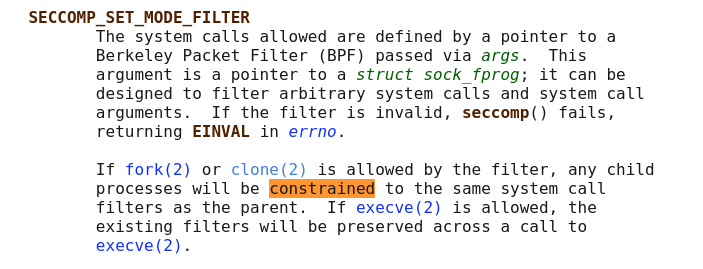
\includegraphics[width=\textwidth]{seccomp_man.png}

    \footnotesize
    \url{https://man7.org/linux/man-pages/man2/seccomp.2.html}
  \end{frame}

  \section{Why normal samples}
  \begin{frame}{Microservices - Riemann sum}
    \centering
    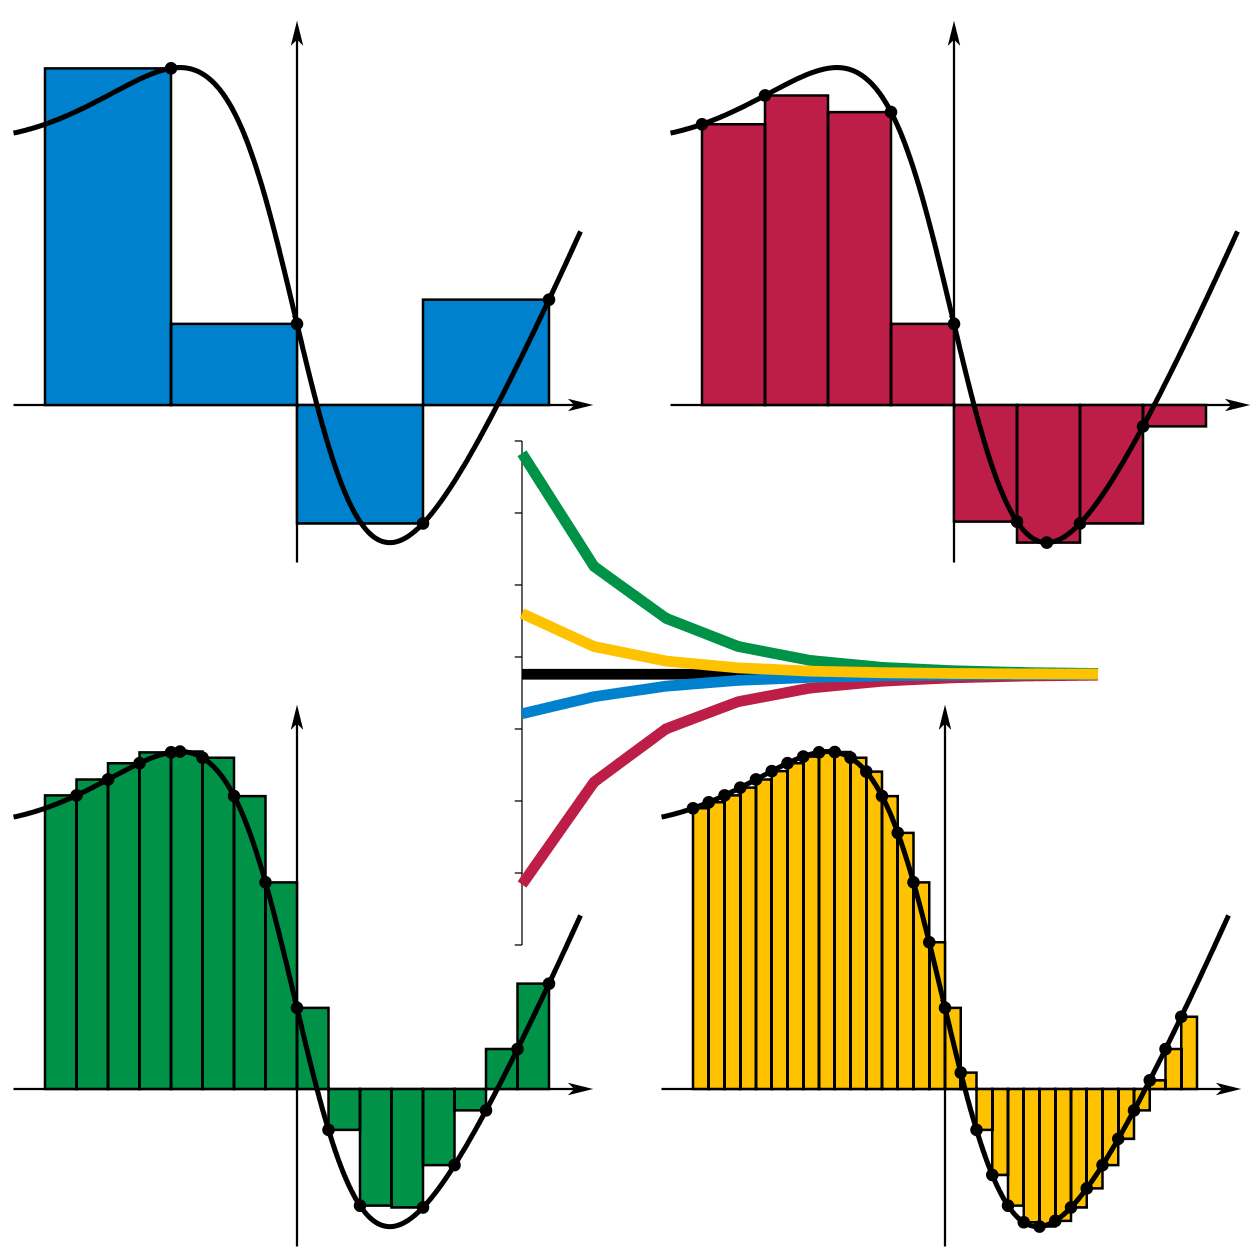
\includegraphics[height=.8\textheight]{Riemann_sum_convergence.png}

    \footnotesize
    \url{https://commons.wikimedia.org/wiki/File:Riemann_sum_convergence.png}
  \end{frame}

  \section{How to find the fine-grained system calls?}
  \begin{frame}{LSMs}
    Might change the kernel. {\color{red} Not inherit}\\
    Profiles and how to write it.
    \begin{itemize}
      \item AppArmor
      \item SELinux
      \item TOMOYO Linux
    \end{itemize}
  \end{frame}

  \begin{frame}{LSMs}
    \begin{itemize}
      \item AppArmor
            \begin{itemize}
              \item Profiles
              \item More fine-grained control in files.
            \end{itemize}
      \item SELinux
            \begin{itemize}
              \item Targeted, Role-Based-Access-Control, Multi-Layer/-Class Security
              \item More fine-grained control in roles.
            \end{itemize}
      \item TOMOYO Linux
    \end{itemize}
  \end{frame}

  \begin{frame}{CGroups}
    \begin{multicols*}{2}
      It seems okay, but might be a little bit tricky to do it.
      \newline
      \hfill
      \newline
      Reading, contributing.
      \newline
      \hfill
      \newline
      Will be published in this weekend AT COSCUP.

      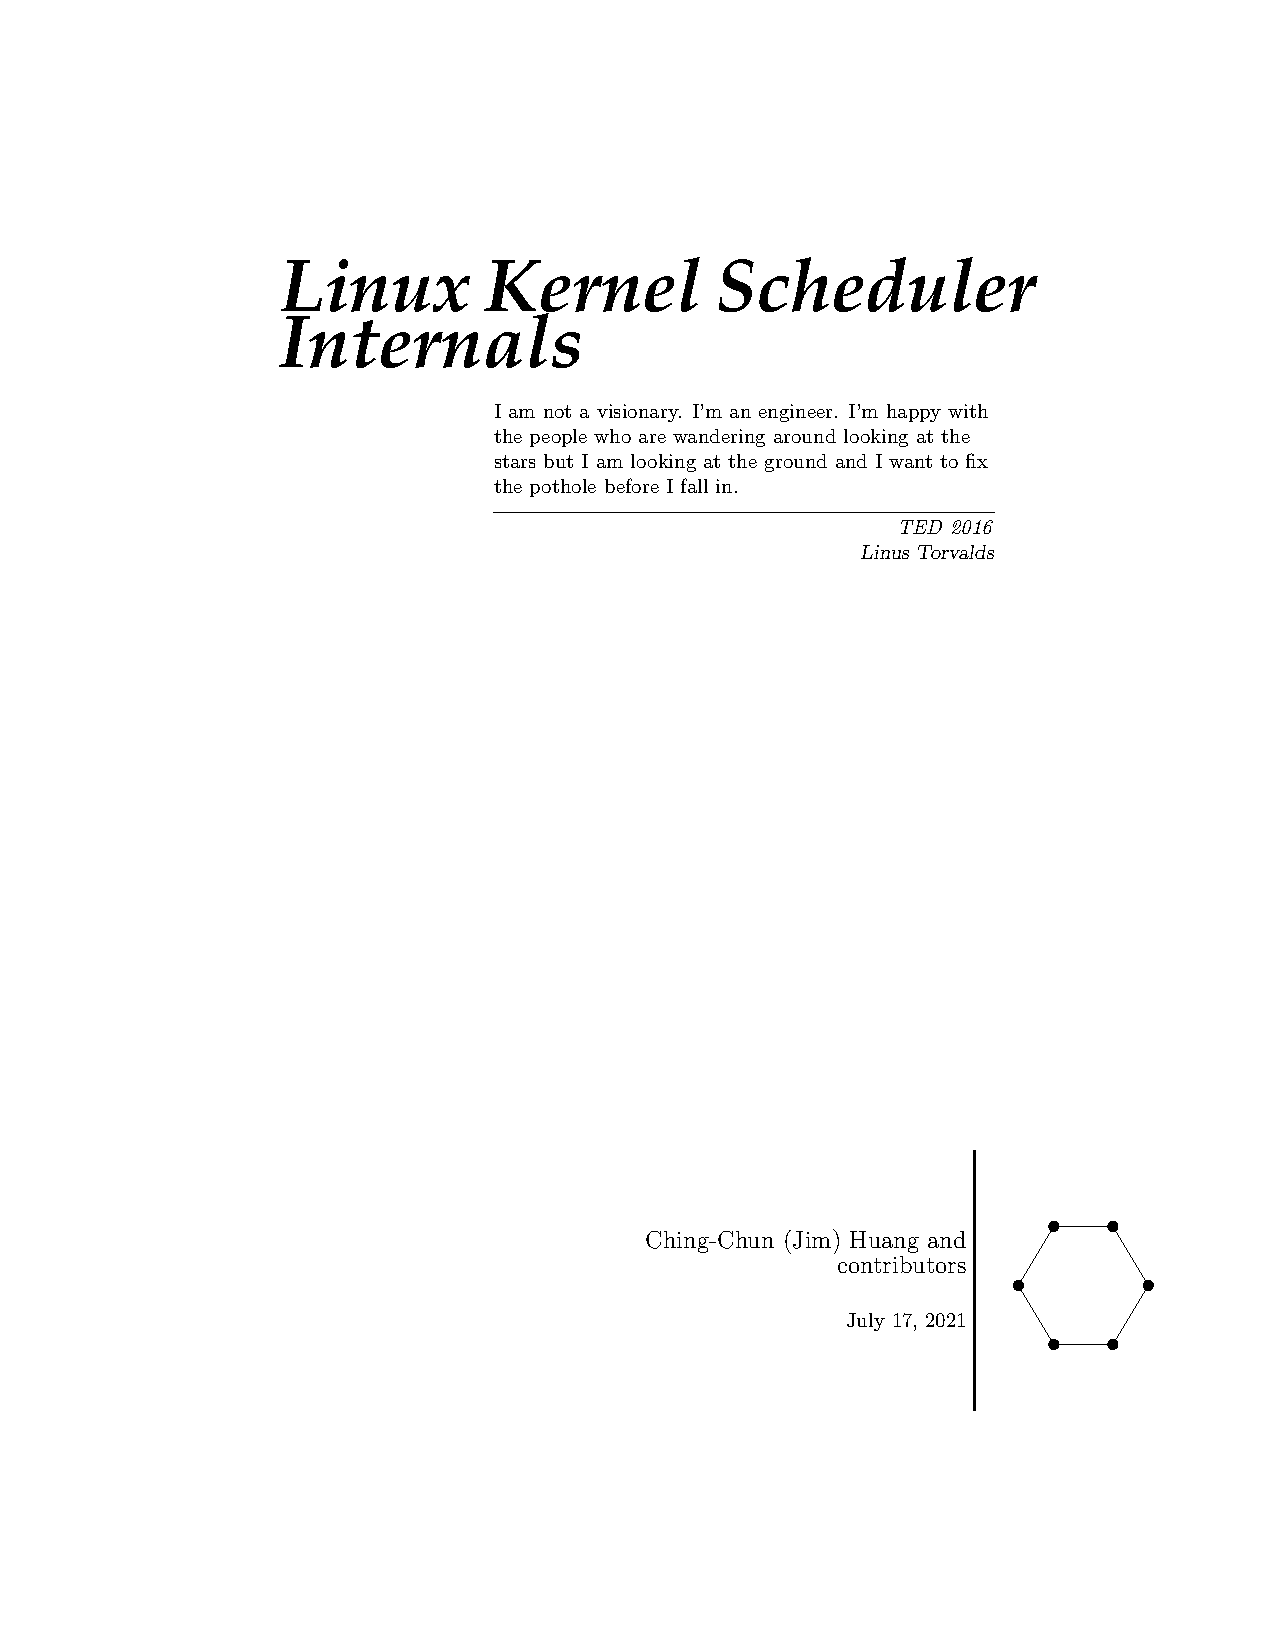
\includegraphics[height=.8\textheight]{src/ksi_cover.pdf}
    \end{multicols*}
  \end{frame}

  \begin{frame}{CGroups}
    There are some people discuss when CGroups named CGroups from `process containers'
    \begin{enumerate}
      \item 2008 \href{http://lkml.iu.edu/hypermail/linux/kernel/0803.1/0671.html}{cgroups: implement device whitelist cgroup\+lsm}
      \item 2011 \href{https://lwn.net/Articles/463636/}{cgroup: syscalls limiting subsystem}
      \item 2011 \href{https://lwn.net/Articles/463683/}{Limiting system calls via control groups?}
    \end{enumerate}
    \begin{quote}{alonz: }
      I wonder if it wouldn't be better to start from the other end of the solution space—small, incremental extensions to seccomp.
    \end{quote}
  \end{frame}

  \begin{frame}{seccomp}
    \begin{itemize}
      \item Advantage
            \begin{itemize}
              \item Inherit
              \item Block by each system call
            \end{itemize}
      \item Disadvantage
            \begin{itemize}
              \item Not cross platforms (CPU architecture)
              \item Custom kernel
            \end{itemize}
    \end{itemize}
  \end{frame}

  \begin{frame}{Papers}
    Intrusion Detection System for Applications Using Linux Containers \cite*{10.1007/978-3-319-24858-5_8}
    \begin{itemize}
      \item Toward Smart Moving Target Defense for Linux Container Resiliency \cite{7796855}
      \item Smart Moving Target Defense for Linux Container Resiliency \cite*{7809699}
      \item Improving the Security of Microservice Systems by Detecting and Tolerating Intrusions \cite*{9307722}
      \item Malchain: Virtual Application Behaviour Profiling by Aggregated Microservice Data Exchange Graph \cite*{9407328}
    \end{itemize}
  \end{frame}

  \begin{frame}{BPF/eBPF}
    \href{https://blog.aquasec.com/ebpf-tracing-containers}{Tracee: Tracing Containers with eBPF}\\
    \href{https://www.youtube.com/watch?v=4SiWL5tULnQ}{DockerCon19 - eBPF Superpowers}\\

    But they are not using in {\color{red} runtime} container security.
  \end{frame}

  \section{Plans}
  \begin{frame}{Plans in next week}
    \begin{itemize}
      \item Use the BPF feature and fuzzing technique to collect the "normal" system calls in healthcare data exchange system.
      \item Keep survey those papers.
    \end{itemize}
  \end{frame}

  \begin{frame}{References}
    \def\bibfont{\footnotesize}
    \printbibliography
  \end{frame}

\end{CJK*}
\end{document}